\chapter{Exemplificando um Apendice}

\section{Gráficos de Resposta em Frequencia Individuais}

\begin{figure}[H]
	\centering 
	\caption{Resposta em Frequencia - FS05XT}
	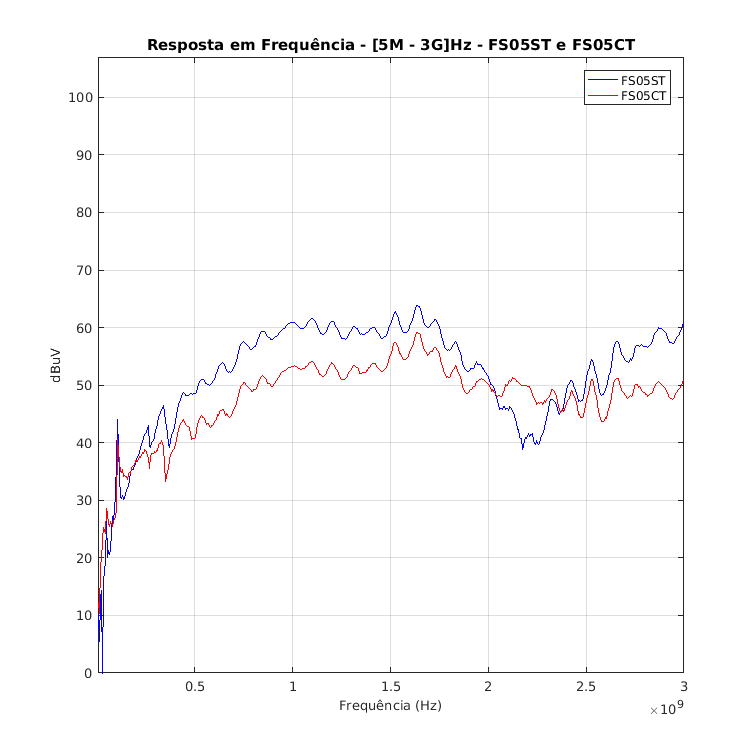
\includegraphics[scale=0.7]{./img/FS05XT}
	\fonte{Elaborado pelo Autor (2019)}
	%\legend{\hspace{-218pt}Fonte:~\citeonline[p.~8]{paul2006}}
	\label{fig:FS05XT}
\end{figure}

\begin{figure}[H]
	\centering 
	\caption{Resposta em Frequencia - FS10XT}
	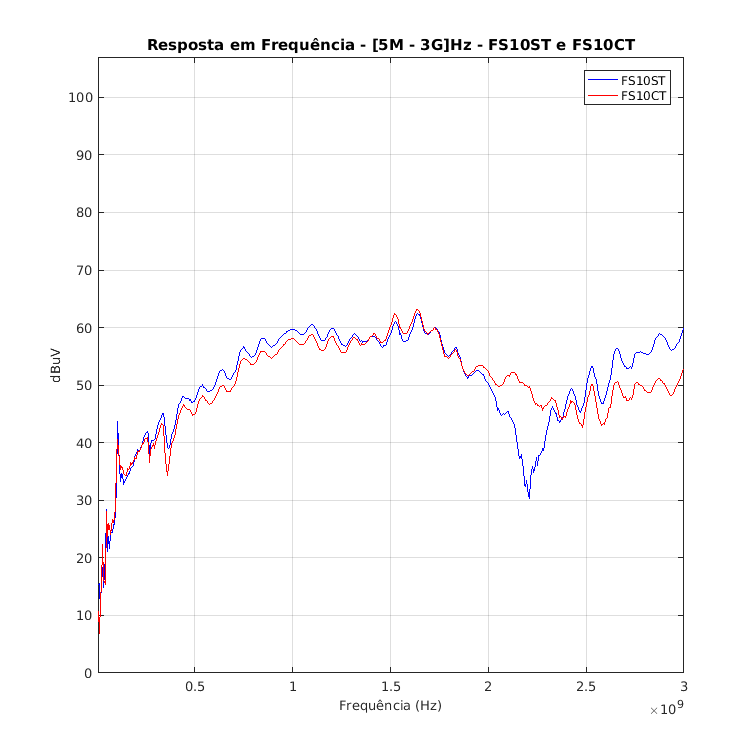
\includegraphics[scale=0.7]{./img/FS10XT}
	\fonte{Elaborado pelo Autor (2019)}
	%\legend{\hspace{-218pt}Fonte:~\citeonline[p.~8]{paul2006}}
	\label{fig:FS10XT}
\end{figure}

\begin{figure}[H]
	\centering 
	\caption{Resposta em Frequencia - FS15XT}
	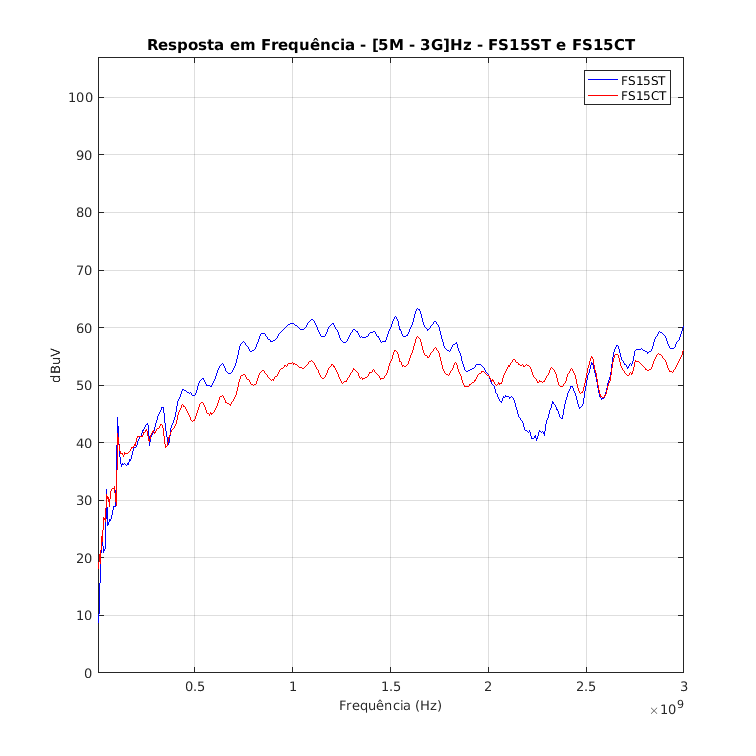
\includegraphics[scale=0.7]{./img/FS15XT}
	\fonte{Elaborado pelo Autor (2019)}
	%\legend{\hspace{-218pt}Fonte:~\citeonline[p.~8]{paul2006}}
	\label{fig:FS15XT}
\end{figure}

\begin{figure}[H]
	\centering 
	\caption{Resposta em Frequencia - FS30XT}
	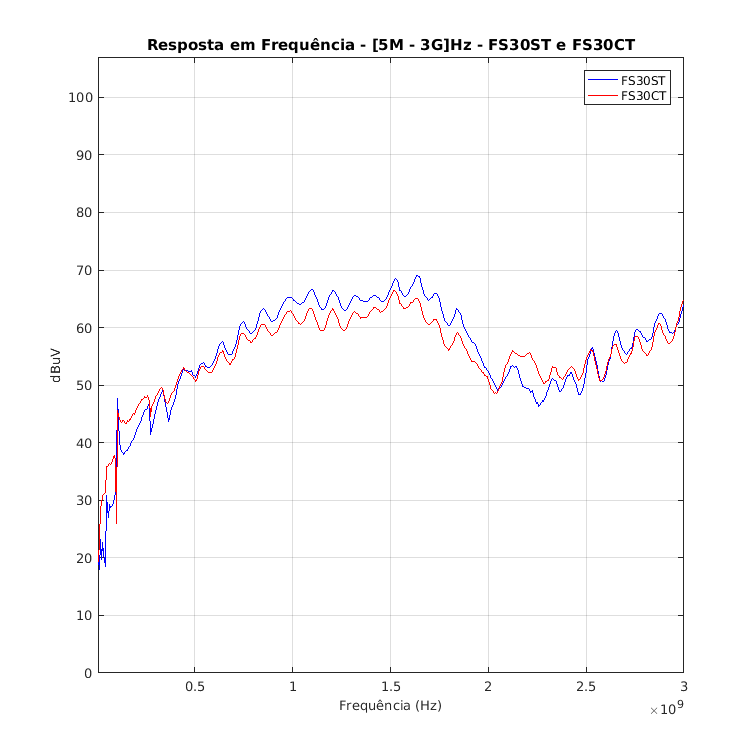
\includegraphics[scale=0.7]{./img/FS30XT}
	\fonte{Elaborado pelo Autor (2019)}
	%\legend{\hspace{-218pt}Fonte:~\citeonline[p.~8]{paul2006}}
	\label{fig:FS30XT}
\end{figure}

\begin{figure}[H]
	\centering 
	\caption{Resposta em Frequencia - FS60XT}
	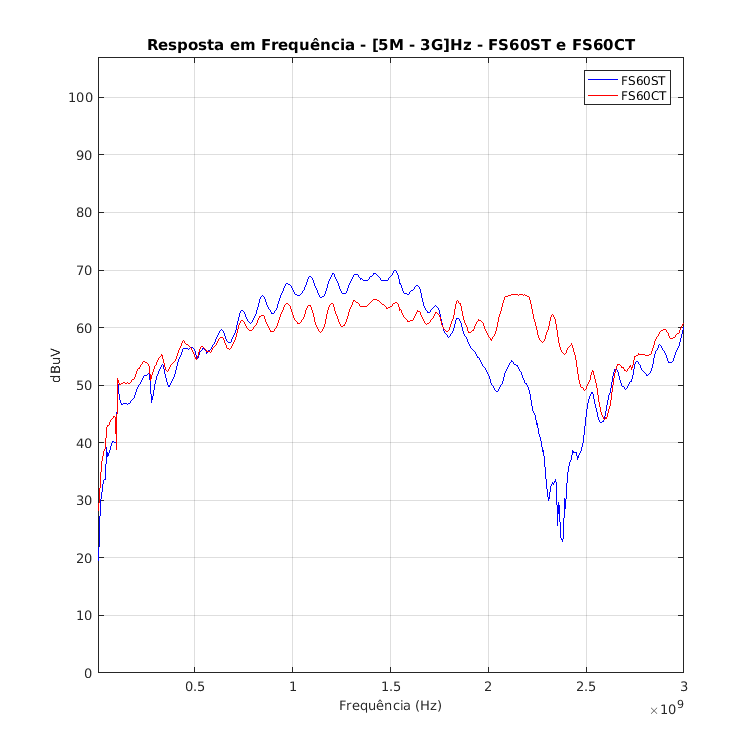
\includegraphics[scale=0.7]{./img/FS60XT}
	\fonte{Elaborado pelo Autor (2019)}
	%\legend{\hspace{-218pt}Fonte:~\citeonline[p.~8]{paul2006}}
	\label{fig:FS60XT}
\end{figure}

%% -------------------------------------- Faces DUPLAS

\begin{figure}[H]
	\centering 
	\caption{Resposta em Frequencia - FD05XT}
	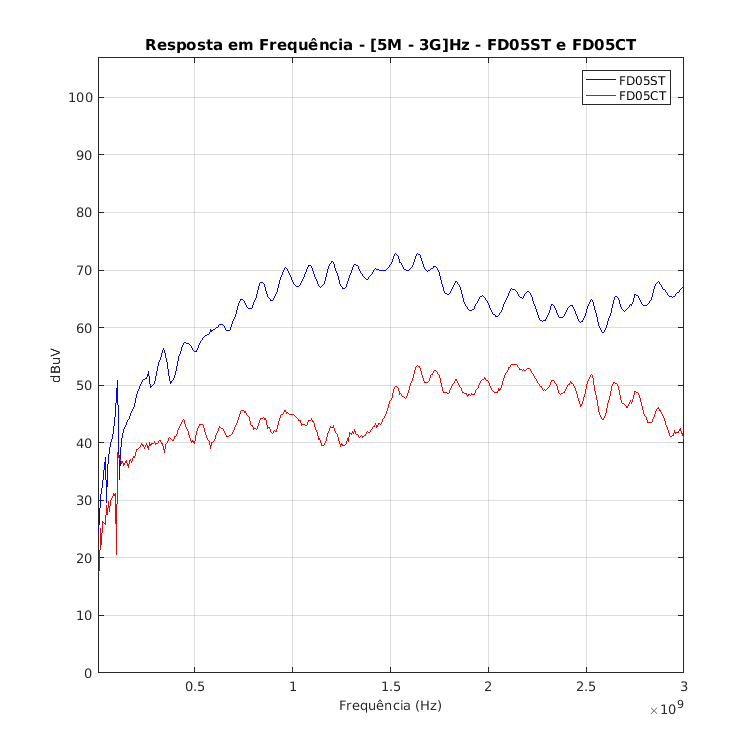
\includegraphics[scale=0.7]{./img/FD05XT}
	\fonte{Elaborado pelo Autor (2019)}
	%\legend{\hspace{-218pt}Fonte:~\citeonline[p.~8]{paul2006}}
	\label{fig:FD05XT}
\end{figure}

\begin{figure}[H]
	\centering 
	\caption{Resposta em Frequencia - FD10XT}
	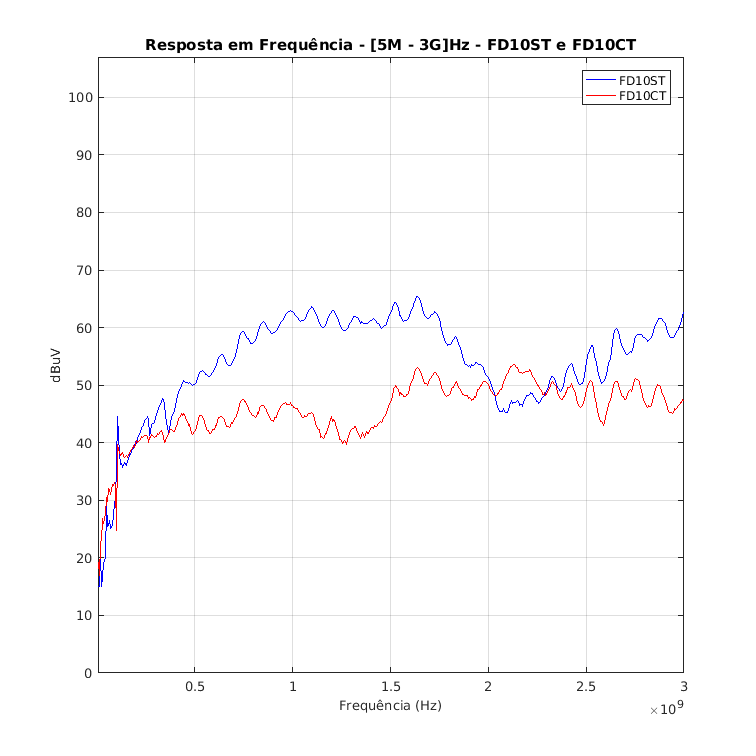
\includegraphics[scale=0.7]{./img/FD10XT}
	\fonte{Elaborado pelo Autor (2019)}
	%\legend{\hspace{-218pt}Fonte:~\citeonline[p.~8]{paul2006}}
	\label{fig:FD10XT}
\end{figure}

\begin{figure}[H]
	\centering 
	\caption{Resposta em Frequencia - FD15XT}
	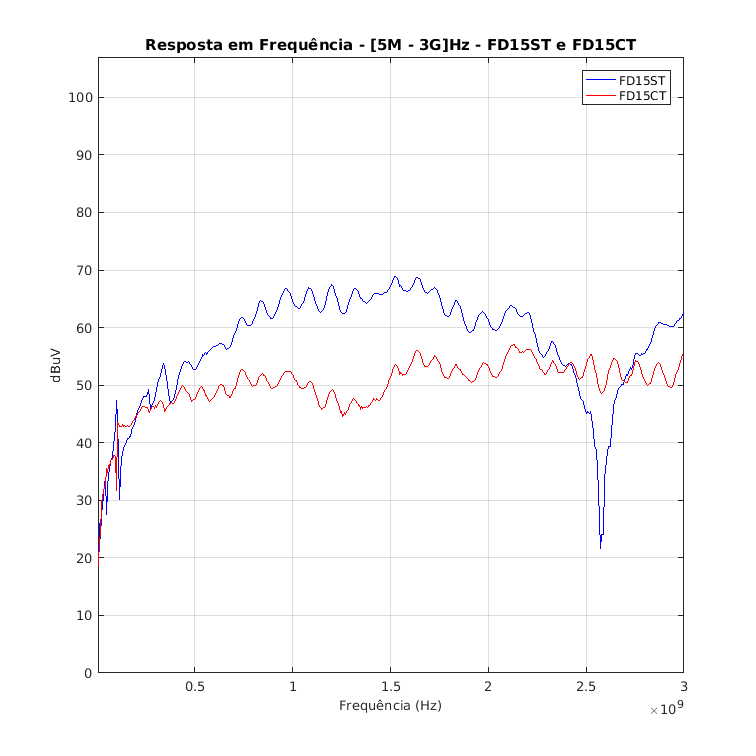
\includegraphics[scale=0.7]{./img/FD15XT}
	\fonte{Elaborado pelo Autor (2019)}
	%\legend{\hspace{-218pt}Fonte:~\citeonline[p.~8]{paul2006}}
	\label{fig:FD15XT}
\end{figure}

\begin{figure}[H]
	\centering 
	\caption{Resposta em Frequencia - FD30XT}
	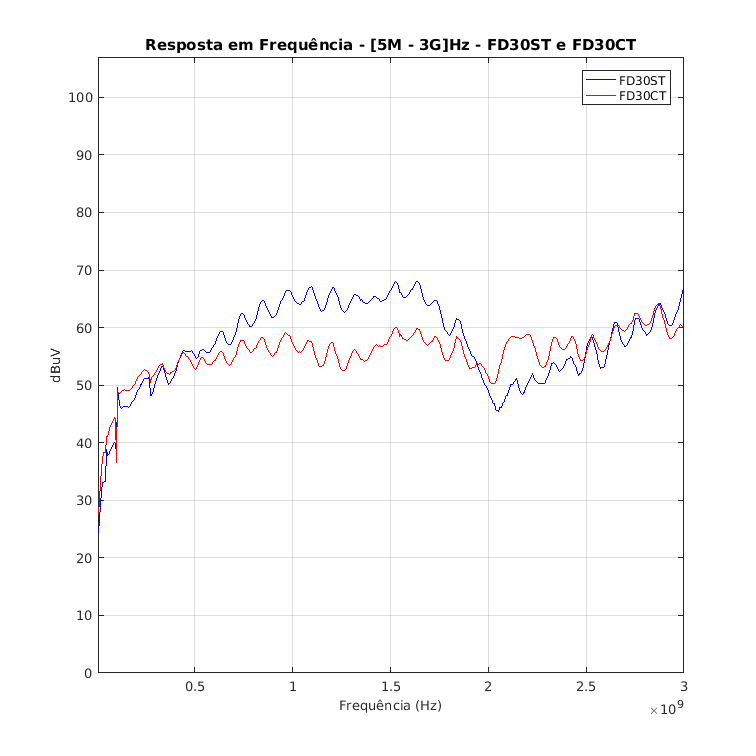
\includegraphics[scale=0.7]{./img/FD30XT}
	\fonte{Elaborado pelo Autor (2019)}
	%\legend{\hspace{-218pt}Fonte:~\citeonline[p.~8]{paul2006}}
	\label{fig:FD30XT}
\end{figure}

\begin{figure}[H]
	\centering 
	\caption{Resposta em Frequencia - FD60XT}
	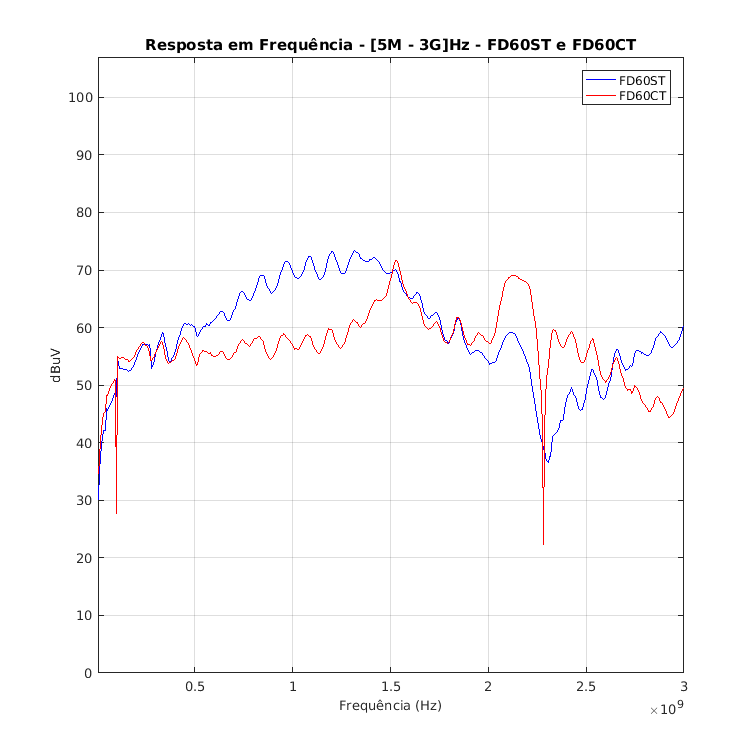
\includegraphics[scale=0.7]{./img/FD60XT}
	\fonte{Elaborado pelo Autor (2019)}
	%\legend{\hspace{-218pt}Fonte:~\citeonline[p.~8]{paul2006}}
	\label{fig:FD60XT}
\end{figure}

\section{Códigos do MatLab - Tratamento dos dados de resposta em frequencia}

\begin{lstlisting}
clear;
clc;

% Import File
% Use the function importfile from matlab
[F,dBuVDUT] = importfile('DUTA_Response.DAT',1, 501);
[F1A,dBuV1A] = importfile('1A_5M-3G.DAT',1, 501);
[F1B,dBuV1B] = importfile('1B_5M-3G.DAT',1, 501);
[F2A,dBuV2A] = importfile('2A_5M-3G.DAT',1, 501);
[F2B,dBuV2B] = importfile('2B_5M-3G.DAT',1, 501);
[F3A,dBuV3A] = importfile('3A_5M-3G.DAT',1, 501);
[F3B,dBuV3B] = importfile('3B_5M-3G.DAT',1, 501);
[F4A,dBuV4A] = importfile('4A_5M-3G.DAT',1, 501);
[F4B,dBuV4B] = importfile('4B_5M-3G.DAT',1, 501);
[F5A,dBuV5A] = importfile('5A_5M-3G.DAT',1, 501);
[F5B,dBuV5B] = importfile('5B_5M-3G.DAT',1, 501);
[F6A,dBuV6A] = importfile('6A_5M-3G.DAT',1, 501);
[F6B,dBuV6B] = importfile('6B_5M-3G.DAT',1, 501);
[F7A,dBuV7A] = importfile('7A_5M-3G.DAT',1, 501);
[F7B,dBuV7B] = importfile('7B_5M-3G.DAT',1, 501);
[F8A,dBuV8A] = importfile('8A_5M-3G.DAT',1, 501);
[F8B,dBuV8B] = importfile('8B_5M-3G.DAT',1, 501);
[F9A,dBuV9A] = importfile('9A_5M-3G.DAT',1, 501);
[F9B,dBuV9B] = importfile('9B_5M-3G.DAT',1, 501);
[F10A,dBuV10A] = importfile('10A_5M-3G.DAT',1, 501);
[F10B,dBuV10B] = importfile('10B_5M-3G.DAT',1, 501);
[FCOM,dBuVCOM] = importfile('COM_5M-3G.DAT',1, 501);

% for remove DC componet
dc1 = dsp.DCBlocker('Algorithm','IIR','Order', 6);
for i = 1:length(dBuVDUT)
      DUT = dc1(dBuVDUT); 
end

dBuV_1A = zeros(length(dBuVDUT),1);
dBuV_1B = zeros(length(dBuVDUT),1);
dBuV_2A = zeros(length(dBuVDUT),1);
dBuV_2B = zeros(length(dBuVDUT),1);
dBuV_3A = zeros(length(dBuVDUT),1);
dBuV_3B = zeros(length(dBuVDUT),1);
dBuV_4A = zeros(length(dBuVDUT),1);
dBuV_4B = zeros(length(dBuVDUT),1);
dBuV_5A = zeros(length(dBuVDUT),1);
dBuV_5B = zeros(length(dBuVDUT),1);
dBuV_6A = zeros(length(dBuVDUT),1);
dBuV_6B = zeros(length(dBuVDUT),1);
dBuV_7A = zeros(length(dBuVDUT),1);
dBuV_7B = zeros(length(dBuVDUT),1);
dBuV_8A = zeros(length(dBuVDUT),1);
dBuV_8B = zeros(length(dBuVDUT),1);
dBuV_9A = zeros(length(dBuVDUT),1);
dBuV_9B = zeros(length(dBuVDUT),1);
dBuV_10A = zeros(length(dBuVDUT),1);
dBuV_10B = zeros(length(dBuVDUT),1);
dBuV_COM = zeros(length(dBuVDUT),1);


for  i = 1:length(dBuVDUT)
    dBuV_1A(i) = dBuV1A(i); % - DUT(i);
    dBuV_1B(i) = dBuV1B(i); % - DUT(i);
    dBuV_2A(i) = dBuV2A(i); % - DUT(i);
    dBuV_2B(i) = dBuV2B(i); % - DUT(i);
    dBuV_3A(i) = dBuV3A(i); % - DUT(i);
    dBuV_3B(i) = dBuV3B(i); % - DUT(i);
    dBuV_4A(i) = dBuV4A(i); % - DUT(i);
    dBuV_4B(i) = dBuV4B(i); % - DUT(i);
    dBuV_5A(i) = dBuV5A(i); % - DUT(i);
    dBuV_5B(i) = dBuV5B(i); % - DUT(i);
    dBuV_6A(i) = dBuV6A(i); % - DUT(i);
    dBuV_6B(i) = dBuV6B(i); % - DUT(i);
    dBuV_7A(i) = dBuV7A(i); % - DUT(i);
    dBuV_7B(i) = dBuV7B(i); % - DUT(i);
    dBuV_8A(i) = dBuV8A(i); % - DUT(i);
    dBuV_8B(i) = dBuV8B(i); % - DUT(i);
    dBuV_9A(i) = dBuV9A(i); % - DUT(i);
    dBuV_9B(i) = dBuV9B(i); % - DUT(i);
    dBuV_10A(i) = dBuV10A(i); % - DUT(i);
    dBuV_10B(i) = dBuV10B(i); % - DUT(i);
    dBuV_COM(i) = dBuVCOM(i); % - DUT(i);
end

%% Graficos 

% f1 = figure('Color', [1 1 1], 'Unit', 'Centimeters', 'Position', [5 5 20 20]);
% a1 = axes('FontName', 'Arial', 'FontSize', 10);
% 
% plot(F,dBuVDUT,'b');
% hold on;
% plot(F,DUT,'-.r');
% grid on;
% 
% title('Resposta em Frequencia - [5M - 3G]Hz - DUT');
% legend('Resposta Natural','IIR 6 - Remove DC','Location','northeast');
% xlabel('Frequencia (Hz)', 'FontName', 'Times', 'FontSize', 10);
% ylabel('dBuV', 'FontName', 'Times', 'FontSize', 10);
% xlim([5e6,3e9]);
% ylim([-10 107]);


f2 = figure('Color', [1 1 1], 'Unit', 'Centimeters', 'Position', [5 5 20 20]);
a2 = axes('FontName', 'Arial', 'FontSize', 10);

plot(F,dBuV_1A,'b');
hold on;
plot(F,dBuV_1B,'r');
grid on;

title('Resposta em Frequencia - [5M - 3G]Hz - FS05ST e FS05CT');
legend('FS05ST','FS05CT','Location','northeast');
xlabel('Frequencia (Hz)', 'FontName', 'Times', 'FontSize', 10);
ylabel('dBuV', 'FontName', 'Times', 'FontSize', 10);
xlim([5e6,3e9]);
ylim([0 107]);

% Demais gráficos seguiram o padrão acima!!

title('Resposta em Frequencia - [5M - 3G]Hz - F?05?T');
legend('FS05ST','FS05CT','FD05ST','FD05CT','Location','northeast');
xlabel('Frequencia (Hz)', 'FontName', 'Times', 'FontSize', 10);
ylabel('dBuV', 'FontName', 'Times', 'FontSize', 10);
xlim([5e6,3e9]);
ylim([0 107]);


f13 = figure('Color', [1 1 1], 'Unit', 'Centimeters', 'Position', [5 5 20 20]);
a13 = axes('FontName', 'Arial', 'FontSize', 10);

plot(F,dBuV_2A,'r');
hold on;
plot(F,dBuV_2B,'-.b');
plot(F,dBuV_5A,'k');
plot(F,dBuV_5B,'-.m');
grid on;

% Demais gráficos seguiram o padrão acima!!

f17 = figure('Color', [1 1 1], 'Unit', 'Centimeters', 'Position', [5 5 20 20]);
a17 = axes('FontName', 'Arial', 'FontSize', 10);

plot(F,dBuV_6B,'b');
hold on;
plot(F,dBuV_7B,'g');
plot(F,dBuV_8B,'k');
plot(F,dBuV_COM,'-.r');
grid on;

title('Resposta em Frequencia - [5M - 3G]Hz - Comparacão com COMERCIAL');
legend('FD15CT','FD30CT','FD60CT','COMERCIAL','Location','northeast');
xlabel('Frequencia (Hz)', 'FontName', 'Times', 'FontSize', 10);
ylabel('dBuV', 'FontName', 'Times', 'FontSize', 10);
xlim([5e6,3e9]);
ylim([0 107]);
\end{lstlisting}

\section{Códigos do MatLab - Tratamento dos dados de intensidade por distancia}
\begin{lstlisting}
clear;
clc;

%% Medidas de dBuV x D
D = [-30 -20 -10 0 10 20 30];         % Distancias em 'mm'
F = [5 10 15 20 25];    % Frequencias em 'MHz'

%% Placa 1
oneA5 = [2413 2617 2923 3215 2923 2617 2413];            
oneA10 = [2744 3073 3602 3825 3602 3073 2744];
oneA15 = [2961 3369 3840 4176 3840 3369 2961];
oneA20 = [3120 3540 3970 4381 3970 3540 3120];
oneA25 = [3297 3726 4047 4590 4047 3726 3297];

oneB5 = [2474 2528 2854 3345 2854 2528 2474];
oneB10 = [2610 2813 3324 3918 3324 2813 2610];
oneB15 = [2826 3084 3696 4240 3696 3084 2826];
oneB20 = [3015 3354 3901 4539 3901 3354 3015];
oneB25 = [3124 3442 4109 4707 4109 3442 3124];

%% Placa 2
twoA5 = [2490 2611 3067 3124 3067 2611 2490];
twoA10 = [2711 3010 3504 3672 3504 3010 2711];
twoA15 = [2930 3284 3840 3977 3840 3284 2930];
twoA20 = [3091 3572 4009 4147 4009 3572 3091];
twoA25 = [3251 3649 4245 4377 4245 3649 3251];

twoB5 = [2506 2617 2843 3558 2843 2617 2506];
twoB10 = [2691 2959 3316 4183 3316 2959 2691];
twoB15 = [2866 3240 3655 4549 3655 3240 2866];
twoB20 = [3040 3464 3988 4761 3988 3464 3040];
twoB25 = [3173 3621 4092 4922 4092 3621 3173];

%% Placa 3
threeA5 = [2509 2761 3296 3433 3296 2761 2509];
threeA10 = [2776 3182 3811 4115 3811 3182 2776];
threeA15 = [3010 3484 4167 4474 4167 3484 3010];
threeA20 = [3251 3688 4396 4707 4396 3688 3251];
threeA25 = [3334 3842 4587 4921 4587 3842 3334];

threeB5 = [2462 2699 2917 4110 2917 2699 2462];
threeB10 = [2716 3014 3515 4676 3515 3014 2716];
threeB15 = [2930 3329 3890 5043 3890 3329 2930];
threeB20 = [3040 3464 4105 5227 4105 3464 3040];
threeB25 = [3240 3711 4340 5477 4340 3711 3240];

%% Placa 4
fourA5 = [2368 2504 3317 4750 3317 2504 2368];
fourA10 = [2513 2759 3904 5152 3904 2759 2513];
fourA15 = [2542 2940 4210 5501 4210 2940 2542];
fourA20 = [2550 3011 4420 5720 4420 3011 2550];
fourA25 = [2560 3095 4580 6090 4580 3095 2560];

fourB5 = [2421 2502 3620 3995 3620 2502 2421];
fourB10 = [2557 2750 3850 4327 3850 2750 2557];
fourB15 = [2646 3033 3911 4722 3911 3033 2646];
fourB20 = [2879 3277 4004 5027 4004 3277 2879];
fourB25 = [2911 3402 4440 5309 4440 3402 2911];

%% Placa 5
fiveA5 = [2422 2490 3550 4854 3550 2490 2422];
fiveA10 = [2594 2671 3644 5328 3644 2671 2594];
fiveA15 = [2890 3020 3628 5650 3628 3020 2890];
fiveA20 = [3031 3118 3832 5862 3832 3118 3031];
fiveA25 = [3267 3380 4041 6038 4041 3380 3267];

fiveB5 = [2412 2509 2823 4018 2823 2509 2412];
fiveB10 = [2513 2772 3243 4577 3243 2772 2513];
fiveB15 = [2688 3042 3591 4944 3591 3042 2688];
fiveB20 = [2753 3244 4001 5174 4001 3244 2753];
fiveB25 = [2977 3418 4004 5377 4004 3418 2977];

%% Placa 6
sixA5 = [2308 2352 2527 4377 2527 2352 2308 ];
sixA10 = [2313 2359 2891 4949 2891 2359 2313];
sixA15 = [2317 2404 3202 5312 3202 2404 2317];
sixA20 = [2321 2442 3380 5540 3380 2442 2321];
sixA25 = [2447 2510 3517 5722 3517 2510 2447];

sixB5 = [2417 2631 3111 4470 3111 2631 2417];
sixB10 = [2597 2973 3715 4753 3715 2973 2597];
sixB15 = [2815 3261 4055 5150 4055 3261 2815];
sixB20 = [2940 3473 4280 5290 4280 3473 2940];
sixB25 = [3180 3677 4477 5677 4477 3677 3180];

%% Placa 7
sevenA5 = [2424 2681 2921 5147 2921 2681 2424];
sevenA10 = [2671 2864 3303 5714 3303 2864 2671];
sevenA15 = [2955 3216 3612 6063 3612 3216 2955];
sevenA20 = [3250 3499 3827 6281 3827 3499 3250];
sevenA25 = [3372 3677 4010 6482 4010 3677 3372];

sevenB5 = [2630 2704 2721 4643 2721 2704 2630];
sevenB10 = [2810 2820 3173 5230 3173 2820 2810];
sevenB15 = [3111 3140 3450 5593 3450 3140 3111];
sevenB20 = [3340 3365 3705 5915 3705 3365 3340];
sevenB25 = [3512 3540 3900 6012 3900 3540 3512];

%% Placa 8
eightA5 = [2822 2981 3267 5274 3267 2981 2822];
eightA10 = [3113 3311 3738 5848 3738 3311 3113];
eightA15 = [3492 3677 4086 6199 4086 3677 3492];
eightA20 = [3769 3925 4335 6421 4335 3925 3769];
eightA25 = [3987 4119 4522 6616 4522 4119 3987];

eightB5 = [2901 3036 3345 5414 3345 3036 2901];
eightB10 = [3363 3455 3866 5990 3866 3455 3363];
eightB15 = [3735 3740 4202 6345 4202 3740 3735];
eightB20 = [3971 3977 4441 6571 4441 3977 3971];
eightB25 = [4171 4170 4631 6770 4631 4170 4171];

%% Placa 9
nineA5 = [2695 2711 3529 5611 3529 2711 2695];
nineA10 = [3391 3015 4042 6184 4042 3015 3391];
nineA15 = [3715 3376 4388 6530 4388 3376 3715];
nineA20 = [3981 3640 4585 6755 4585 3640 3981];
nineA25 = [4173 3841 4781 6948 4781 3841 4173];

nineB5 = [3092 3239 3907 5472 3907 3239 3092];
nineB10 = [3671 3844 4550 6054 4550 3844 3671];
nineB15 = [4027 4206 4897 6405 4897 4206 4027];
nineB20 = [4269 4444 5113 6631 5113 4444 4269];
nineB25 = [4462 4637 5284 6826 5284 4637 4462];

%% Placa 10
tenA5 = [3500 3548 4268 5901 4268 3548 3500];
tenA10 = [3974 4146 4871 6479 4871 4146 3874];
tenA15 = [4357 4518 5216 6829 5216 4518 4357];
tenA20 = [4600 4763 5431 7051 5431 4763 4600];
tenA25 = [4792 4964 5625 7243 5625 4964 4792];

tenB5 = [3552 3815 4387 5981 4387 3815 3552];
tenB10 = [4212 4384 4955 6564 4955 4384 4212];
tenB15 = [4558 4743 5305 6914 5305 4743 4558];
tenB20 = [4787 4979 5527 7138 5527 4979 4787];
tenB25 = [4977 5166 5724 7332 5724 5166 4977];

%% Medidas com DUT duplo - Resolucão Espacial

RefA = [-10 -20 -30 -40 -50];   % Distancia relativa ao DUT (A) em 'mm'
fDUT_A = 20;                    % Frequencia do sinal imposta no DUT (A) em 'MHz'
fDUT_B = 25;                    % Frequencia do sinal imposta no DUT (B) em 'MHz'
    
oneArefA = [3931 3540 3120 2777 2674];      % Medida da intensidade em 20MHz - refA
oneArefB = [2790 2901 3310 3777 3982];      % Medida da intensidade em 25MHz - refB

oneBrefA = [3779 3354 3015 2681 2518];
oneBrefB = [2715 2915 3188 3677 3846];


twoArefA = [4009 3572 3091 2761 2681];
twoArefB = [2744 2950 3312 3737 4091];

twoBrefA = [3988 3464 3040 2768 2550];
twoBrefB = [2737 2917 3572 3674 4093];


threeArefA = [4176 3688 3251 2871 2669];
threeArefB = [2840 3140 3475 3964 4345];

threeBrefA = [3961 3559 3045 2765 2563];
threeBrefB = [2762 3077 3418 3842 4108];


fourArefA = [4501 3249 2970 2790 2042];
fourArefB = [2480 2440 2420 2906 4235];

fourBrefA = [3556 3277 2879 2618 2545];
fourBrefB = [2754 2891 3060 3473 3840];


fiveArefA = [4416 3817 3417 3018 2770];
fiveArefB = [2915 3141 3498 3997 4460];

fiveBrefA = [4001 3241 2753 2510 2461];
fiveBrefB = [2533 2672 2894 3346 3907];


sixArefA = [3480 2477 2471 2455 2446];
sixArefB = [2484 2402 2418 3253 4052];

sixBrefA = [4503 3650 3033 2719 2520];
sixBrefB = [2767 2867 3310 3675 4201];

sevenArefA = [3827 3499 3250 2963 2766];
sevenArefB = [2890 3099 3413 3791 4010];

sevenBrefA = [3705 3365 3340 3051 2816];
sevenBrefB = [2949 3191 3512 3540 3900];

eightArefA = [4335 3769 3607 3548 3330];
eightArefB = [3469 3745 3987 4119 4522];

eightBrefA = [4441 3977 3971 3682 3320];
eightBrefB = [3512 3804 4171 4170 4631];

nineArefA = [4585 3640 3981 3850 3615];
nineArefB = [3790 4015 4173 3841 4781];

nineBrefA = [5113 4444 4269 3950 3670];
nineBrefB = [3815 4090 4462 4637 5284];

tenArefA = [5431 4763 4600 4407 4172];
tenArefB = [4373 4594 4792 4964 5625];

tenBrefA = [5527 4979 4787 4521 4230];
tenBrefB = [4438 4650 4977 5166 5724];


%% Matrizes Completas
oneA = [oneA5;oneA10;oneA15;oneA20;oneA25];
oneB = [oneB5;oneB10;oneB15;oneB20;oneB25];

twoA = [twoA5;twoA10;twoA15;twoA20;twoA25];
twoB = [twoB5;twoB10;twoB15;twoB20;twoB25];

threeA = [threeA5;threeA10;threeA15;threeA20;threeA25];
threeB = [threeB5;threeB10;threeB15;threeB20;threeB25];

fourA = [fourA5;fourA10;fourA15;fourA20;fourA25];
fourB = [fourB5;fourB10;fourB15;fourB20;fourB25];

fiveA = [fiveA5;fiveA10;fiveA15;fiveA20;fiveA25];
fiveB = [fiveB5;fiveB10;fiveB15;fiveB20;fiveB25];

sixA = [sixA5;sixA10;sixA15;sixA20;sixA25];
sixB = [sixB5;sixB10;sixB15;sixB20;sixB25];


%% Resultados
%% mm(Lateral) x dBuv
% --------------------------------------------------------------------------------------------------
% ------------- NFP 1A

f1 = figure('Color', [1 1 1], 'Unit', 'Centimeters', 'Position', [5 5 20 20]);
a1 = axes('FontName', 'Arial', 'FontSize', 10);

%Interpolacoes
xD =[-50:1:50];
xoneA5 = interp1(D,oneA5,xD,'pchip');
xoneA10 = interp1(D,oneA10,xD,'pchip');
xoneA15 = interp1(D,oneA15,xD,'pchip');
xoneA20 = interp1(D,oneA20,xD,'pchip');
xoneA25 = interp1(D,oneA25,xD,'pchip');

plot(D,oneA5./100,'*r',D,oneA10./100,'og',D,oneA15./100,'+b',D,oneA20./100,'xc',D,oneA25./100,'pm');
hold on;
plot(xD(1,20:80),xoneA5(1,20:80)./100,'-.r');
plot(xD(1,20:80),xoneA10(1,20:80)./100,'-.g');
plot(xD(1,20:80),xoneA15(1,20:80)./100,'-.b');
plot(xD(1,20:80),xoneA20(1,20:80)./100,'-.c');
plot(xD(1,20:80),xoneA25(1,20:80)./100,'-.m');
grid on;

title('mm (Lateral) x dBuV - FS05ST');
legend('5MHz','10MHz','15MHz','20MHz','25MHz');
xlabel('Distancia (mm)', 'FontName', 'Times', 'FontSize', 10);
ylabel('dBuV', 'FontName', 'Times', 'FontSize', 10);
xlim([-50,50]);
ylim([0 75]);

% Demais gráficos seguiram o padrão acima!!

%% DUT Duplo - Single Face

f21 = figure('Color', [1 1 1], 'Unit', 'Centimeters', 'Position', [5 5 40 40]);
a21 = axes('FontName', 'Arial', 'FontSize', 10);

subplot(2,5,1);
% Interpolacoes
xRefA = [0:-1:-60];
xoneArefA = interp1(RefA,oneArefA,xRefA,'spline');
xoneArefB = interp1(RefA,oneArefB,xRefA,'spline');

plot(RefA,oneArefA./100,'*r');
hold on;
plot(RefA,oneArefB./100,'ob');

plot(xRefA(1,1:49),xoneArefA(1,1:49)./100,'-.r');
plot(xRefA(1,10:60),xoneArefB(1,10:60)./100,'-.b');
grid on;

title('DUT Duplo - FS05ST');
legend('20MHz','25MHz','Interpolados','Location','southeast');
xlabel('Distancia (mm)', 'FontName', 'Times', 'FontSize', 10);
ylabel('dBuV', 'FontName', 'Times', 'FontSize', 10);
xlim([-50,-10]);
ylim([0 75]);


subplot(2,5,6);
% Interpolacoes
xoneBrefA = interp1(RefA,oneBrefA,xRefA,'spline');
xoneBrefB = interp1(RefA,oneBrefB,xRefA,'spline');

plot(RefA,oneBrefA./100,'*r');
hold on;
plot(RefA,oneBrefB./100,'ob');

plot(xRefA(1,1:49),xoneBrefA(1,1:49)./100,'-.r');
plot(xRefA(1,10:60),xoneBrefB(1,10:60)./100,'-.b');
grid on;

title('DUT Duplo - FS05CT');
legend('20MHz','25MHz','Interpolados','Location','southeast');
xlabel('Distancia (mm)', 'FontName', 'Times', 'FontSize', 10);
ylabel('dBuV', 'FontName', 'Times', 'FontSize', 10);
xlim([-50,-10]);
ylim([0 75]);


subplot(2,5,2);
% Interpolacoes
xRefA = [0:-1:-60];
xtwoArefA = interp1(RefA,twoArefA,xRefA,'spline');
xtwoArefB = interp1(RefA,twoArefB,xRefA,'spline');

plot(RefA,twoArefA./100,'*r');
hold on;
plot(RefA,twoArefB./100,'ob');

plot(xRefA(1,1:49),xtwoArefA(1,1:49)./100,'-.r');
plot(xRefA(1,10:60),xtwoArefB(1,10:60)./100,'-.b');
grid on;

title('DUT Duplo - FS10ST');
legend('20MHz','25MHz','Interpolados','Location','southeast');
xlabel('Distancia (mm)', 'FontName', 'Times', 'FontSize', 10);
ylabel('dBuV', 'FontName', 'Times', 'FontSize', 10);
xlim([-50,-10]);
ylim([0 75]);


subplot(2,5,7);
% Interpolacoes
xRefA = [0:-1:-60];
xtwoBrefA = interp1(RefA,twoBrefA,xRefA,'spline');
xtwoBrefB = interp1(RefA,twoBrefB,xRefA,'spline');

plot(RefA,twoBrefA./100,'*r');
hold on;
plot(RefA,twoBrefB./100,'ob');

plot(xRefA(1,1:49),xtwoBrefA(1,1:49)./100,'-.r');
plot(xRefA(1,10:60),xtwoBrefB(1,10:60)./100,'-.b');
grid on;

title('DUT Duplo - FS10CT');
legend('20MHz','25MHz','Interpolados','Location','southeast');
xlabel('Distancia (mm)', 'FontName', 'Times', 'FontSize', 10);
ylabel('dBuV', 'FontName', 'Times', 'FontSize', 10);
xlim([-50,-10]);
ylim([0 75]);


subplot(2,5,3);
% Interpolacoes
xRefA = [0:-1:-60];
xthreeArefA = interp1(RefA,threeArefA,xRefA,'spline');
xthreeArefB = interp1(RefA,threeArefB,xRefA,'spline');

plot(RefA,threeArefA./100,'*r');
hold on;
plot(RefA,threeArefB./100,'ob');

plot(xRefA(1,1:49),xthreeArefA(1,1:49)./100,'-.r');
plot(xRefA(1,10:60),xthreeArefB(1,10:60)./100,'-.b');
grid on;

title('DUT Duplo - FS15ST');
legend('20MHz','25MHz','Interpolados','Location','southeast');
xlabel('Distancia (mm)', 'FontName', 'Times', 'FontSize', 10);
ylabel('dBuV', 'FontName', 'Times', 'FontSize', 10);
xlim([-50,-10]);
ylim([0 75]);


subplot(2,5,8);
% Interpolacoes
xRefA = [0:-1:-60];
xthreeBrefA = interp1(RefA,threeBrefA,xRefA,'spline');
xthreeBrefB = interp1(RefA,threeBrefB,xRefA,'spline');

plot(RefA,threeBrefA./100,'*r');
hold on;
plot(RefA,threeBrefB./100,'ob');

plot(xRefA(1,1:49),xthreeBrefA(1,1:49)./100,'-.r');
plot(xRefA(1,10:60),xthreeBrefB(1,10:60)./100,'-.b');
grid on;

title('DUT Duplo - FS15CT');
legend('20MHz','25MHz','Interpolados','Location','southeast');
xlabel('Distancia (mm)', 'FontName', 'Times', 'FontSize', 10);
ylabel('dBuV', 'FontName', 'Times', 'FontSize', 10);
xlim([-50,-10]);
ylim([0 75]);


subplot(2,5,4);
% Interpolacoes
xRefA = [0:-1:-60];
xsevenArefA = interp1(RefA,sevenArefA,xRefA,'spline');
xsevenArefB = interp1(RefA,sevenArefB,xRefA,'spline');

plot(RefA,sevenArefA./100,'*r');
hold on;
plot(RefA,sevenArefB./100,'ob');

plot(xRefA(1,1:49),xsevenArefA(1,1:49)./100,'-.r');
plot(xRefA(1,10:60),xsevenArefB(1,10:60)./100,'-.b');
grid on;

title('DUT Duplo - FS30ST');
legend('20MHz','25MHz','Interpolados','Location','southeast');
xlabel('Distancia (mm)', 'FontName', 'Times', 'FontSize', 10);
ylabel('dBuV', 'FontName', 'Times', 'FontSize', 10);
xlim([-50,-10]);
ylim([0 75]);


subplot(2,5,9);
% Interpolacoes
xRefA = [0:-1:-60];
xsevenBrefA = interp1(RefA,sevenBrefA,xRefA,'spline');
xsevenBrefB = interp1(RefA,sevenBrefB,xRefA,'spline');

plot(RefA,sevenBrefA./100,'*r');
hold on;
plot(RefA,sevenBrefB./100,'ob');

plot(xRefA(1,1:49),xsevenBrefA(1,1:49)./100,'-.r');
plot(xRefA(1,10:60),xsevenBrefB(1,10:60)./100,'-.b');
grid on;

title('DUT Duplo - FS30CT');
legend('20MHz','25MHz','Interpolados','Location','southeast');
xlabel('Distancia (mm)', 'FontName', 'Times', 'FontSize', 10);
ylabel('dBuV', 'FontName', 'Times', 'FontSize', 10);
xlim([-50,-10]);
ylim([0 75]);

subplot(2,5,5);
% Interpolacoes
xRefA = [0:-1:-60];
xnineArefA = interp1(RefA,nineArefA,xRefA,'spline');
xnineArefB = interp1(RefA,nineArefB,xRefA,'spline');

plot(RefA,nineArefA./100,'*r');
hold on;
plot(RefA,nineArefB./100,'ob');

plot(xRefA(1,1:49),xnineArefA(1,1:49)./100,'-.r');
plot(xRefA(1,10:60),xnineArefB(1,10:60)./100,'-.b');
grid on;

title('DUT Duplo - FS60ST');
legend('20MHz','25MHz','Interpolados','Location','southeast');
xlabel('Distancia (mm)', 'FontName', 'Times', 'FontSize', 10);
ylabel('dBuV', 'FontName', 'Times', 'FontSize', 10);
xlim([-50,-10]);
ylim([0 75]);

subplot(2,5,10);
% Interpolacoes
xRefA = [0:-1:-60];
xnineBrefA = interp1(RefA,nineBrefA,xRefA,'spline');
xnineBrefB = interp1(RefA,nineBrefB,xRefA,'spline');

plot(RefA,nineBrefA./100,'*r');
hold on;
plot(RefA,nineBrefB./100,'ob');

plot(xRefA(1,1:49),xnineBrefA(1,1:49)./100,'-.r');
plot(xRefA(1,10:60),xnineBrefB(1,10:60)./100,'-.b');
grid on;

title('DUT Duplo - FS60CT');
legend('20MHz','25MHz','Interpolados','Location','southeast');
xlabel('Distancia (mm)', 'FontName', 'Times', 'FontSize', 10);
ylabel('dBuV', 'FontName', 'Times', 'FontSize', 10);
xlim([-50,-10]);
ylim([0 75]);


%% DUT Duplo - Double Face

f22 = figure('Color', [1 1 1], 'Unit', 'Centimeters', 'Position', [5 5 40 40]);
a22 = axes('FontName', 'Arial', 'FontSize', 10);

subplot(2,5,1);
% Interpolacoes
xRefA = [0:-1:-60];
xfourArefA = interp1(RefA,fourArefA,xRefA,'spline');
xfourArefB = interp1(RefA,fourArefB,xRefA,'spline');

plot(RefA,fourArefA./100,'*r');
hold on;
plot(RefA,fourArefB./100,'ob');

plot(xRefA(1,1:49),xfourArefA(1,1:49)./100,'-.r');
plot(xRefA(1,10:60),xfourArefB(1,10:60)./100,'-.b');
grid on;

title('DUT Duplo - FD05ST');
legend('20MHz','25MHz','Interpolados','Location','southeast');
xlabel('Distancia (mm)', 'FontName', 'Times', 'FontSize', 10);
ylabel('dBuV', 'FontName', 'Times', 'FontSize', 10);
xlim([-50,-10]);
ylim([0 75]);


subplot(2,5,6);
% Interpolacoes
xRefA = [0:-1:-60];
xfourBrefA = interp1(RefA,fourBrefA,xRefA,'spline');
xfourBrefB = interp1(RefA,fourBrefB,xRefA,'spline');

plot(RefA,fourBrefA./100,'*r');
hold on;
plot(RefA,fourBrefB./100,'ob');

plot(xRefA(1,1:49),xfourBrefA(1,1:49)./100,'-.r');
plot(xRefA(1,10:60),xfourBrefB(1,10:60)./100,'-.b');
grid on;

title('DUT Duplo - FD05CT');
legend('20MHz','25MHz','Interpolados','Location','southeast');
xlabel('Distancia (mm)', 'FontName', 'Times', 'FontSize', 10);
ylabel('dBuV', 'FontName', 'Times', 'FontSize', 10);
xlim([-50,-10]);
ylim([0 75]);


subplot(2,5,2);
% Interpolacoes
xRefA = [0:-1:-60];
xfiveArefA = interp1(RefA,fiveArefA,xRefA,'spline');
xfiveArefB = interp1(RefA,fiveArefB,xRefA,'spline');

plot(RefA,fiveArefA./100,'*r');
hold on;
plot(RefA,fiveArefB./100,'ob');

plot(xRefA(1,1:49),xfiveArefA(1,1:49)./100,'-.r');
plot(xRefA(1,10:60),xfiveArefB(1,10:60)./100,'-.b');
grid on;

title('DUT Duplo - FD10ST');
legend('20MHz','25MHz','Interpolados','Location','southeast');
xlabel('Distancia (mm)', 'FontName', 'Times', 'FontSize', 10);
ylabel('dBuV', 'FontName', 'Times', 'FontSize', 10);
xlim([-50,-10]);
ylim([0 75]);


subplot(2,5,7);
% Interpolacoes
xRefA = [0:-1:-60];
xfiveBrefA = interp1(RefA,fiveBrefA,xRefA,'spline');
xfiveBrefB = interp1(RefA,fiveBrefB,xRefA,'spline');

plot(RefA,fiveBrefA./100,'*r');
hold on;
plot(RefA,fiveBrefB./100,'ob');

plot(xRefA(1,1:49),xfiveBrefA(1,1:49)./100,'-.r');
plot(xRefA(1,10:60),xfiveBrefB(1,10:60)./100,'-.b');
grid on;

title('DUT Duplo - FD10CT');
legend('20MHz','25MHz','Interpolados','Location','southeast');
xlabel('Distancia (mm)', 'FontName', 'Times', 'FontSize', 10);
ylabel('dBuV', 'FontName', 'Times', 'FontSize', 10);
xlim([-50,-10]);
ylim([0 75]);


subplot(2,5,3);
% Interpolacoes
xRefA = [0:-1:-60];
xsixArefA = interp1(RefA,sixArefA,xRefA,'spline');
xsixArefB = interp1(RefA,sixArefB,xRefA,'spline');

plot(RefA,sixArefA./100,'*r');
hold on;
plot(RefA,sixArefB./100,'ob');

plot(xRefA(1,1:49),xsixArefA(1,1:49)./100,'-.r');
plot(xRefA(1,10:60),xsixArefB(1,10:60)./100,'-.b');
grid on;

title('DUT Duplo - FD15ST');
legend('20MHz','25MHz','Interpolados','Location','southeast');
xlabel('Distancia (mm)', 'FontName', 'Times', 'FontSize', 10);
ylabel('dBuV', 'FontName', 'Times', 'FontSize', 10);
xlim([-50,-10]);
ylim([0 75]);


subplot(2,5,8);
% Interpolacoes
xRefA = [0:-1:-60];
xsixBrefA = interp1(RefA,sixBrefA,xRefA,'spline');
xsixBrefB = interp1(RefA,sixBrefB,xRefA,'spline');

plot(RefA,sixBrefA./100,'*r');
hold on;
plot(RefA,sixBrefB./100,'ob');

plot(xRefA(1,1:49),xsixBrefA(1,1:49)./100,'-.r');
plot(xRefA(1,10:60),xsixBrefB(1,10:60)./100,'-.b');
grid on;

title('DUT Duplo - FD15CT');
legend('20MHz','25MHz','Interpolados','Location','southeast');
xlabel('Distancia (mm)', 'FontName', 'Times', 'FontSize', 10);
ylabel('dBuV', 'FontName', 'Times', 'FontSize', 10);
xlim([-50,-10]);
ylim([0 75]);


subplot(2,5,4);
% Interpolacoes
xRefA = [0:-1:-60];
xeightArefA = interp1(RefA,eightArefA,xRefA,'spline');
xeightArefB = interp1(RefA,eightArefB,xRefA,'spline');

plot(RefA,eightArefA./100,'*r');
hold on;
plot(RefA,eightArefB./100,'ob');

plot(xRefA(1,1:49),xeightArefA(1,1:49)./100,'-.r');
plot(xRefA(1,10:60),xeightArefB(1,10:60)./100,'-.b');
grid on;

title('DUT Duplo - FD30ST');
legend('20MHz','25MHz','Interpolados','Location','southeast');
xlabel('Distancia (mm)', 'FontName', 'Times', 'FontSize', 10);
ylabel('dBuV', 'FontName', 'Times', 'FontSize', 10);
xlim([-50,-10]);
ylim([0 75]);


subplot(2,5,9);
% Interpolacoes
xRefA = [0:-1:-60];
xeightBrefA = interp1(RefA,eightBrefA,xRefA,'spline');
xeightBrefB = interp1(RefA,eightBrefB,xRefA,'spline');

plot(RefA,eightBrefA./100,'*r');
hold on;
plot(RefA,eightBrefB./100,'ob');

plot(xRefA(1,1:49),xeightBrefA(1,1:49)./100,'-.r');
plot(xRefA(1,10:60),xeightBrefB(1,10:60)./100,'-.b');
grid on;

title('DUT Duplo - FD30CT');
legend('20MHz','25MHz','Interpolados','Location','southeast');
xlabel('Distancia (mm)', 'FontName', 'Times', 'FontSize', 10);
ylabel('dBuV', 'FontName', 'Times', 'FontSize', 10);
xlim([-50,-10]);
ylim([0 75]);

subplot(2,5,5);
% Interpolacoes
xRefA = [0:-1:-60];
xtenArefA = interp1(RefA,tenArefA,xRefA,'spline');
xtenArefB = interp1(RefA,tenArefB,xRefA,'spline');

plot(RefA,tenArefA./100,'*r');
hold on;
plot(RefA,tenArefB./100,'ob');

plot(xRefA(1,1:49),xtenArefA(1,1:49)./100,'-.r');
plot(xRefA(1,10:60),xtenArefB(1,10:60)./100,'-.b');
grid on;

title('DUT Duplo - FD60ST');
legend('20MHz','25MHz','Interpolados','Location','southeast');
xlabel('Distancia (mm)', 'FontName', 'Times', 'FontSize', 10);
ylabel('dBuV', 'FontName', 'Times', 'FontSize', 10);
xlim([-50,-10]);
ylim([0 75]);

subplot(2,5,10);
% Interpolacoes
xRefA = [0:-1:-60];
xtenBrefA = interp1(RefA,tenBrefA,xRefA,'spline');
xtenBrefB = interp1(RefA,tenBrefB,xRefA,'spline');

plot(RefA,tenBrefA./100,'*r');
hold on;
plot(RefA,tenBrefB./100,'ob');

plot(xRefA(1,1:49),xtenBrefA(1,1:49)./100,'-.r');
plot(xRefA(1,10:60),xtenBrefB(1,10:60)./100,'-.b');
grid on;

title('DUT Duplo - FD60CT');
legend('20MHz','25MHz','Interpolados','Location','southeast');
xlabel('Distancia (mm)', 'FontName', 'Times', 'FontSize', 10);
ylabel('dBuV', 'FontName', 'Times', 'FontSize', 10);
xlim([-50,-10]);
ylim([0 75]);


%% Frequencia versus NFP

f23 = figure('Color', [1 1 1], 'Unit', 'Centimeters', 'Position', [5 5 20 20]);
a23 = axes('FontName', 'Arial', 'FontSize', 10);

subplot(2,1,1);
plot(D,oneA5./100,'*r',D,twoA5./100,'og',D,threeA5./100,'+b',D,sevenA5./100,'xc',D,nineA5./100,'pm');
hold on;
plot(xD(1,20:80),xoneA5(1,20:80)./100,'-.r');
plot(xD(1,20:80),xtwoA5(1,20:80)./100,'-.g');
plot(xD(1,20:80),xthreeA5(1,20:80)./100,'-.b');
plot(xD(1,20:80),xsevenA5(1,20:80)./100,'-.c');
plot(xD(1,20:80),xnineA5(1,20:80)./100,'-.m');
grid on;

title('mm (Lateral) x dBuV - FSxxST (5MHz)');
legend('FS05ST','FS10ST','FS15ST','FS30ST','FS60ST');
xlabel('Distancia (mm)', 'FontName', 'Times', 'FontSize', 10);
ylabel('dBuV', 'FontName', 'Times', 'FontSize', 10);
xlim([-50,50]);
ylim([0 75]);

subplot(2,1,2);
plot(D,oneB5./100,'*r',D,twoB5./100,'og',D,threeB5./100,'+b',D,sevenB5./100,'xc',D,nineB5./100,'pm');
hold on;
plot(xD(1,20:80),xoneB5(1,20:80)./100,'-.r');
plot(xD(1,20:80),xtwoB5(1,20:80)./100,'-.g');
plot(xD(1,20:80),xthreeB5(1,20:80)./100,'-.b');
plot(xD(1,20:80),xsevenB5(1,20:80)./100,'-.c');
plot(xD(1,20:80),xnineB5(1,20:80)./100,'-.m');
grid on;

title('mm (Lateral) x dBuV - FSxxCT (5MHz)');
legend('FS05CT','FS10CT','FS15CT','FS30CT','FS60CT');
xlabel('Distancia (mm)', 'FontName', 'Times', 'FontSize', 10);
ylabel('dBuV', 'FontName', 'Times', 'FontSize', 10);
xlim([-50,50]);
ylim([0 75]);

% Demais gráficos seguiram o padrão acima!!

\end{lstlisting}

\section{Códigos do MatLab - Calculos de Tensão e Campos no DUT e NFP}
\begin{lstlisting}
clear;
clc;

%Constantes
c = 300e+6; %m/s (Velocidade da Luz)
mu0 = pi*4e-7; % H/m (Permeabilidade no Vácuo)
eps0 = 8.8541878176e-12; % F/m (Permissividade do Vácuo)
epsFR4 = 4.4; % F/m (Permissividade do FR-4)


%% ANALISANDO O DUT - Campo Próximo ou Distante
D = 0.1; % 10cm de comprimento
f = 25e+6; % 25MHz

lambda = (c/f);

%Campo Prximo Reativo (Reactive Near Field)
%                   D^3
% R < 0.62 * sqrt(-------)
%                  lambda

Reativo = 0.62*sqrt(D^3/lambda);

%Campo Próximo Radiativo (Radiating Near Field (Fresnel Region)
%          D^2
% R < 2* --------
%         lambda         

Radiativo = 2*(D^2/lambda);

%Campo Distante
%          D^2
% R > 2* --------
%         lambda   


%Tensão Aplicada no DUT(A)
V = 1; % Vp
R = 50; % Ohm
f = 25e+6; % 25MHz
rd = 1e-3; % 1mm - Distância do Fio

I = V/R;    % Corrente de Pico
B = mu0*I/2*pi*rd; % T (Tesla) - Densidade Magnética Pico
H = B/mu0; % A/m (Amperes por Metro) --> Campo Magnético (Pico) acima do DUT em 'rd' distante

%% ANALISANDO AS NFP - Tensão Lida e Campo Magnético
% Caso para FD15ST 
%f = 5e+6:1e+6:3e+9;
%lambda = (c./f);

% Parametros Contrutivos
raio = 0.0015; % 1.5mm - Raio da FS15ST
N = 2;          % Numero de Espiras
A = pi*raio;    % Area da Espira
W = 2*pi*f;     % Frequencia Angular

circ = 2*pi*raio;
diam = 2*raio;

% Para ser Eletricamente Pequena deve-se atender aos critérios
% Condição de Diametro
% diam < 0.01*lambda

% Condicação de Circumferência -- Antena Eletricamente Pequena
% circ < 0.1*lambda 

% figure(1)
% plot(0.1*lambda);

V = W*mu0*H*N*A; % Tensão na Espira

% 10^[(dBμV−120)/20] = V
% dBuV = 120 + 20log(V)
dBuV = 120 + 20*log10(V); %dBuV

% FUNÇÂO DE TRANFERÊNCIA
tr = 0.5e-3; % 20mils ou 0.508mm --> Aproximção do raio da trilha

L = mu0*raio*log(raio/tr);
C = (2*epsFR4*eps0*raio)/(log(raio/tr));

W0 = 1/(sqrt(L*C));
Q = R*W0*C;
sigma = W/W0;

for i=1:length(f)
    FT(i) = W(i)*mu0*N*A*abs(1/(1/Q + j*(sigma(i)-1/sigma(i))));
end

% FATOR DE ANTENA
AF = 1./(j*W*mu0*N*A);

figure(2)
plot(f,FT,'r')
hold on
%plot(f,abs(AF))
plot(f,dBuV,'-.b')
\end{lstlisting}
